\documentclass[12pt]{article}
\usepackage[utf8]{inputenc}
\usepackage{geometry}
\geometry{a4paper, margin=0.8in}
\usepackage{graphicx}
\usepackage{booktabs}
\usepackage{caption}
\usepackage{tabularx} % For adjustable table width
\usepackage{amsmath}
\usepackage{amsfonts}
\usepackage{hyperref}
\usepackage{xcolor}
\usepackage{enumitem}
\usepackage{float}
\usepackage{lipsum} % For placeholder text (remove in final version)

\begin{document}

\section{Problem 4: Impact of Attention Mechanisms in Deep Learning}

This section explores the transformative role of attention mechanisms in enhancing neural network performance across two distinct recognition tasks: digit classification and audio recognition. The analysis is divided into two complementary parts: Part A investigates visual recognition through the Reduced MNIST dataset, while Part B examines audio-based recognition via spectrograms of spoken digits. 

\section{Part A: Understanding the Profound Impact of Attention Mechanisms on Reduced MNIST Classification}

\subsection{Introduction}
The Reduced MNIST dataset, a thoughtfully curated subset of the iconic MNIST collection, comprises grayscale images of handwritten digits (0-9), each meticulously rendered at a resolution of 28x28 pixels and organized by class. This project represents a significant evolution from prior assignments, aiming to harness the power of attention mechanisms to elevate the classification prowess of CNNs. \\
\\
This study embarks on a detailed exploration of how attention mechanisms transform the performance of Convolutional Neural Networks (CNNs) for classifying handwritten digits. Five meticulously crafted models were developed and rigorously evaluated: a foundational Base CNN, a CNN augmented with Spatial Attention, a CNN enriched with Self-Attention, a CNN fortified with the Convolutional Block Attention Module (CBAM) incorporating both channel and spatial attention, and a CNN optimized with Squeeze-and-Excitation (SE) Channel Attention. Each model incorporated a dropout rate of 0.3 to mitigate overfitting, a critical regularization strategy given the dataset's characteristics. The standout performer, the CNN with SE Channel Attention, achieved an impressive test accuracy of 0.9855, surpassing the Base CNN's 0.9810, while the Self-Attention CNN lagged at 0.9820. Training times varied significantly, with the Self-Attention model requiring a substantial 80.55 seconds due to its computational intensity.\\
\\
The primary objectives are multifaceted:
\begin{itemize}
    \item \textbf{Develop a Base CNN}: Establish a robust baseline model, building upon the foundational LeNet-inspired architecture, to serve as a reference point for performance evaluation.
    \item \textbf{Implement Diverse Attention Mechanisms}: Integrate a suite of attention strategies—Spatial Attention, Self-Attention, CBAM (channel and spatial attention), and SE Channel Attention—into CNN frameworks, each designed to refine feature focus and enhance decision-making.
    \item \textbf{Conduct Comparative Analysis}: Rigorously compare these models in terms of classification accuracy and training time, providing a quantitative assessment of their efficacy.
    \item \textbf{Visualize Attention Impact}: Leverage attention maps to offer visual insights into the regions of digit images that each model prioritizes, bridging the gap between numerical results and interpretability.\\
\end{itemize}

\newpage
\subsection{Methodology}

\subsubsection{Dataset and Preprocessing}
The Reduced MNIST dataset, a distilled version of the original MNIST collection, was meticulously loaded from directory structures, with images organized by digit class (0-9). This dataset, comprising 5000 training images and 1000 test images, was preprocessed with precision to optimize CNN performance. Each grayscale image, originally 28x28 pixels, was normalized to the range [0, 1] by dividing pixel values by 255, ensuring compatibility with neural network activation functions and promoting stable gradient flow. The images were reshaped to (28, 28, 1) to accommodate the CNN input requirements, preserving the single-channel nature of grayscale data. A random seed of 4 was employed to shuffle the dataset, guaranteeing reproducibility across experiments and maintaining a consistent evaluation framework. The resulting dataset shapes are:
\begin{itemize}
    \item \textbf{Training Images}: (5000, 28, 28, 1), representing a diverse array of handwritten digit samples.
    \item \textbf{Training Labels}: (5000,), integer-encoded class labels from 0 to 9.
    \item \textbf{Testing Images}: (1000, 28, 28, 1), a held-out set for final evaluation.
    \item \textbf{Testing Labels}: (1000,), corresponding class labels.
\end{itemize}
This preprocessing pipeline laid a solid foundation, ensuring the data was primed for the intricate feature extraction processes of the subsequent models.

\subsubsection{Network Architectures}
Five distinct CNN models were engineered using TensorFlow and Keras, each infused with a dropout rate of 0.3 after the dense layer to mitigate overfitting—a critical consideration given the dataset's moderate size and the risk of memorizing training patterns. The architectures, tailored to exploit the 28x28x1 input, are detailed below and summarized in Table \ref{tab:architectures} for clarity and comparison.

\paragraph{Base CNN}
The Base CNN serves as the foundational benchmark, drawing inspiration from the classic LeNet architecture, renowned for its success in digit classification tasks. This model adopts a straightforward yet effective design to extract hierarchical features from handwritten digits:
\begin{itemize}
    \item \textbf{Input Layer}: Accepts 28x28x1 grayscale images, capturing the raw pixel intensities of each digit.
    \item \textbf{First Convolutional Block}:
        \begin{itemize}
            \item \textbf{Conv2D}: Applies 32 filters with a 3x3 kernel and ReLU activation, reducing spatial dimensions to 26x26x32. This layer detects low-level features such as edges and corners, forming the building blocks of digit shapes.
            \item \textbf{MaxPooling2D}: Employs a 2x2 pool with stride 2, downsampling to 13x13x32, halving the spatial dimensions while retaining the most prominent features, thus reducing computational complexity.
        \end{itemize}
    \item \textbf{Second Convolutional Block}:
        \begin{itemize}
            \item \textbf{Conv2D}: Increases to 64 filters, 3x3 kernel, with ReLU, outputting 11x11x64. This layer captures more complex patterns, such as loops or intersections, essential for distinguishing digits like "8" or "0".
            \item \textbf{MaxPooling2D}: Another 2x2 pool, reducing to 5x5x64, further condensing the feature representation.
        \end{itemize}
    \item \textbf{Fully Connected Layers}:
        \begin{itemize}
            \item \textbf{Flatten}: Transforms the 5x5x64 feature map into a 1600-dimensional vector, preparing it for classification.
            \item \textbf{Dense}: 128 units with ReLU activation, serving as a hidden layer to model high-level abstractions and refine feature combinations.
            \item \textbf{Dropout}: Applies a 0.3 dropout rate, randomly deactivating 30\% of units during training to prevent co-adaptation and enhance generalization.
            \item \textbf{Dense}: 10 units with softmax activation, producing a probability distribution over the 10 digit classes.
        \end{itemize}
\end{itemize}
This architecture, with approximately 200,000 parameters, leverages a simple yet powerful structure to achieve high baseline performance, setting the stage for attention-enhanced variants.

\paragraph{CNN with Spatial Attention}
The CNN with Spatial Attention extends the base model by introducing a spatial attention mechanism, designed to emphasize spatially significant regions within the digit images:
\begin{itemize}
    \item \textbf{Input Layer}: 28x28x1 grayscale images.
    \item \textbf{First Convolutional Block}:
        \begin{itemize}
            \item \textbf{Conv2D}: 32 filters, 3x3, ReLU, outputs 26x26x32.
            \item \textbf{MaxPooling2D}: 2x2 pool, outputs 13x13x32.
        \end{itemize}
    \item \textbf{Spatial Attention}:
        \begin{itemize}
            \item \textbf{Conv2D}: 1 filter, 1x1 kernel, sigmoid activation, applied to the feature map to generate spatial weights.
            \item \textbf{Multiply}: Weights the 13x13x32 feature map, highlighting regions like digit strokes or curves (e.g., loops of '8' or the bar of '1').
        \end{itemize}
    \item \textbf{Second Convolutional Block}:
        \begin{itemize}
            \item \textbf{Conv2D}: 64 filters, 3x3, ReLU, outputs 11x11x64.
            \item \textbf{MaxPooling2D}: 2x2 pool, outputs 5x5x64.
        \end{itemize}
    \item \textbf{Fully Connected Layers}: Identical to the base model (Flatten, Dense(128), Dropout(0.3), Dense(10)).
\end{itemize}
The spatial attention adds approximately 1000 parameters, focusing the model on key spatial areas, though its impact is tempered by the dataset's simplicity.

\paragraph{CNN with Self-Attention}
The CNN with Self-Attention introduces a transformer-inspired approach, leveraging multi-head attention to model long-range dependencies within the feature maps:
\begin{itemize}
    \item \textbf{Input Layer}: 28x28x1 grayscale images.
    \item \textbf{First Convolutional Block}:
        \begin{itemize}
            \item \textbf{Conv2D}: 32 filters, 3x3, ReLU, outputs 26x26x32.
            \item \textbf{MaxPooling2D}: 2x2 pool, outputs 13x13x32.
        \end{itemize}
    \item \textbf{Second Convolutional Block}:
        \begin{itemize}
            \item \textbf{Conv2D}: 64 filters, 3x3, ReLU, outputs 11x11x64.
            \item \textbf{MaxPooling2D}: 2x2 pool, outputs 5x5x64.
        \end{itemize}
    \item \textbf{Self-Attention}:
        \begin{itemize}
            \item \textbf{Reshape}: Transforms 5x5x64 to (25, 64) for 5x5 patches, treating each patch as a token for attention computation.
            \item \textbf{MultiHeadAttention}: 4 heads, key dimension 64, captures relationships between patches across the image.
            \item \textbf{LayerNormalization}: Stabilizes the attention output, ensuring consistent feature scaling.
        \end{itemize}
    \item \textbf{Fully Connected Layers}: Same as base model.
\end{itemize}
This model adds approximately 50,000 parameters due to the attention heads, aiming to model global dependencies, though its complexity proved less effective for the compact Reduced MNIST images.

\paragraph{CNN with CBAM}
The CNN with CBAM integrates the full Convolutional Block Attention Module \cite{cbam_paper}, combining channel and spatial attention for a holistic feature refinement:
\begin{itemize}
    \item \textbf{Input Layer}: 28x28x1 grayscale images.
    \item \textbf{First Convolutional Block}:
        \begin{itemize}
            \item \textbf{Conv2D}: 32 filters, 3x3, ReLU, outputs 26x26x32.
            \item \textbf{MaxPooling2D}: 2x2 pool, outputs 13x13x32.
        \end{itemize}
    \item \textbf{CBAM}:
        \begin{itemize}
            \item \textbf{Channel Attention}: Global average pooling summarizes spatial data, followed by two dense layers (reduction ratio 8, sigmoid activation) to weight channels, emphasizing frequency-like features.
            \item \textbf{Spatial Attention}: 7x7 convolution on concatenated average/max-pooled maps generates spatial weights, highlighting regions like the vertical stroke of '1'.
            \item \textbf{Multiply}: Applies weights to refine the 13x13x32 feature map.
        \end{itemize}
    \item \textbf{Second Convolutional Block}:
        \begin{itemize}
            \item \textbf{Conv2D}: 64 filters, 3x3, ReLU, outputs 11x11x64.
            \item \textbf{MaxPooling2D}: 2x2 pool, outputs 5x5x64.
        \end{itemize}
    \item \textbf{Fully Connected Layers}: Same as base model.
\end{itemize}
CBAM adds approximately 2000 parameters, offering a dual focus that enhances feature relevance but increases computational cost.

\paragraph{CNN with SE Channel Attention}
The CNN with SE Channel Attention employs the Squeeze-and-Excitation (SE) module \cite{se_paper}, a lightweight channel attention mechanism:
\begin{itemize}
    \item \textbf{Input Layer}: 28x28x1 grayscale images.
    \item \textbf{First Convolutional Block}:
        \begin{itemize}
            \item \textbf{Conv2D}: 32 filters, 3x3, ReLU, outputs 26x26x32.
            \item \textbf{MaxPooling2D}: 2x2 pool, outputs 13x13x32.
        \end{itemize}
    \item \textbf{SE Module}:
        \begin{itemize}
            \item \textbf{Global Average Pooling}: Summarizes spatial information into a channel descriptor.
            \item \textbf{Dense}: 4 units, ReLU, reduces dimensionality for efficiency.
            \item \textbf{Dense}: 32 units, sigmoid, generates channel weights.
            \item \textbf{Scale}: Applies weights to refine the 13x13x32 feature map, emphasizing discriminative features like edges.
        \end{itemize}
    \item \textbf{Second Convolutional Block}:
        \begin{itemize}
            \item \textbf{Conv2D}: 64 filters, 3x3, ReLU, outputs 11x11x64.
            \item \textbf{MaxPooling2D}: 2x2 pool, outputs 5x5x64.
        \end{itemize}
    \item \textbf{Fully Connected Layers}: Same as base model.
\end{itemize}
The SE module adds approximately 500 parameters, offering an efficient channel weighting strategy that proved highly effective.

\begin{table}[H]
    \centering
    \caption{Part 1: Network Architectures for Reduced MNIST Classification Models (Base and Spatial Attention)}
    \label{tab:architectures_part1}
    \begin{tabularx}{\textwidth}{l X}
        \toprule
        \textbf{Model} & \textbf{Architecture} \\
        \midrule
        Base CNN & 
        \begin{itemize}
            \item \textbf{Input Layer}: 28x28x1 grayscale images.
            \item \textbf{First Convolutional Block}: Conv2D(32, 3$\times$3, ReLU) $\rightarrow$ MaxPooling2D(2$\times$2) to 13x13x32, detecting edges and basic shapes.
            \item \textbf{Second Convolutional Block}: Conv2D(64, 3$\times$3, ReLU) $\rightarrow$ MaxPooling2D(2$\times$2) to 5x5x64, capturing complex patterns like loops.
            \item \textbf{Fully Connected Layers}: Flatten to 1600 $\rightarrow$ Dense(128, ReLU) $\rightarrow$ Dropout(0.3) $\rightarrow$ Dense(10, Softmax).
        \end{itemize} \\
        \midrule
        CNN with Spatial Attention & 
        \begin{itemize}
            \item \textbf{Input Layer}: 28x28x1 grayscale images.
            \item \textbf{First Convolutional Block}: Conv2D(32, 3$\times$3, ReLU) $\rightarrow$ MaxPooling2D(2$\times$2) to 13x13x32.
            \item \textbf{Spatial Attention}: Conv2D(1, 1$\times$1, Sigmoid) $\rightarrow$ Multiply with feature maps, emphasizing digit strokes (e.g., '8' loops).
            \item \textbf{Second Convolutional Block}: Conv2D(64, 3$\times$3, ReLU) $\rightarrow$ MaxPooling2D(2$\times$2) to 5x5x64.
            \item \textbf{Fully Connected Layers}: Same as base model.
        \end{itemize} \\
        \bottomrule
    \end{tabularx}
\end{table}

\begin{table}[H]
    \centering
    \caption{Part 2: Network Architectures for Reduced MNIST Classification Models (Self-Attention, CBAM, and SE Channel Attention)}
    \label{tab:architectures_part2}
    \begin{tabularx}{\textwidth}{l X}
        \toprule
        \textbf{Model} & \textbf{Architecture} \\
        \midrule
        CNN with Self-Attention & 
        \begin{itemize}
            \item \textbf{Input Layer}: 28x28x1 grayscale images.
            \item \textbf{First Convolutional Block}: Conv2D(32, 3$\times$3, ReLU) $\rightarrow$ MaxPooling2D(2$\times$2) to 13x13x32.
            \item \textbf{Second Convolutional Block}: Conv2D(64, 3$\times$3, ReLU) $\rightarrow$ MaxPooling2D(2$\times$2) to 5x5x64.
            \item \textbf{Self-Attention}: Reshape to (25, 64) for 5$\times$5 patches $\rightarrow$ MultiHeadAttention(4 heads, key dim=64) $\rightarrow$ LayerNormalization, modeling global dependencies.
            \item \textbf{Fully Connected Layers}: Same as base model.
        \end{itemize} \\
        \midrule
        CNN with CBAM & 
        \begin{itemize}
            \item \textbf{Input Layer}: 28x28x1 grayscale images.
            \item \textbf{First Convolutional Block}: Conv2D(32, 3$\times$3, ReLU) $\rightarrow$ MaxPooling2D(2$\times$2) to 13x13x32.
            \item \textbf{CBAM}: Channel Attention (Global Pooling + MLP) weights frequency features $\rightarrow$ Spatial Attention (7x7 Conv) highlights spatial regions (e.g., '1' stroke).
            \item \textbf{Second Convolutional Block}: Conv2D(64, 3$\times$3, ReLU) $\rightarrow$ MaxPooling2D(2$\times$2) to 5x5x64.
            \item \textbf{Fully Connected Layers}: Same as base model.
        \end{itemize} \\
        \midrule
        CNN with SE Channel Attention & 
        \begin{itemize}
            \item \textbf{Input Layer}: 28x28x1 grayscale images.
            \item \textbf{First Convolutional Block}: Conv2D(32, 3$\times$3, ReLU) $\rightarrow$ MaxPooling2D(2$\times$2) to 13x13x32.
            \item \textbf{SE Module}: Global Average Pooling $\rightarrow$ Dense(4, ReLU) $\rightarrow$ Dense(32, Sigmoid) $\rightarrow$ Scale, reweighting channels for key features (e.g., edges).
            \item \textbf{Second Convolutional Block}: Conv2D(64, 3$\times$3, ReLU) $\rightarrow$ MaxPooling2D(2$\times$2) to 5x5x64.
            \item \textbf{Fully Connected Layers}: Same as base model.
        \end{itemize} \\
        \bottomrule
    \end{tabularx}
\end{table}

\subsubsection{Training Process and Hyperparameters}
All models underwent a standardized training regimen to ensure a fair and equitable comparison, with hyperparameters meticulously chosen to optimize performance while addressing potential pitfalls. The details are encapsulated in Table \ref{tab:hyperparameters}, and the process is elaborated below to provide a comprehensive understanding.

\paragraph{Training Procedure}
The training was conducted in a controlled environment, enforcing CPU computation by setting the \texttt{CUDA\_VISIBLE\_DEVICES} environment variable to an empty string. This decision ensured consistency across models, though it sacrificed speed for reliable benchmarking, a trade-off deemed acceptable given the assignment's focus on comparison. Training times were meticulously recorded using Python's \texttt{time} module, capturing the duration from the first epoch to the last. The test set, comprising 1000 images, doubled as the validation set to monitor performance dynamically during training, providing immediate feedback on generalization and enabling real-time adjustments. Each model was trained for 10 epochs, a duration determined through preliminary runs where convergence was typically achieved within 8-10 epochs, balancing thorough learning with computational efficiency.

\paragraph{Hyperparameter Selection}
The hyperparameter configuration was a result of iterative experimentation, balancing model capacity, regularization, and computational efficiency:
\begin{itemize}
    \item \textbf{Optimizer}: The Adam optimizer was selected for its adaptive learning rate properties, utilizing default settings to ensure broad applicability across models. This choice facilitated stable convergence without requiring extensive tuning, allowing the models to adapt to the varying complexities introduced by attention mechanisms.
    \item \textbf{Loss Function}: Sparse categorical crossentropy was employed, aligning perfectly with the multi-class classification task. This loss function computes the cross-entropy loss between true integer labels and predicted probability distributions, providing a robust metric for backpropagation across the 10 digit classes, ensuring accurate error propagation.
    \item \textbf{Epochs}: Set to 10, this number was chosen based on initial trials where models converged within 8-10 epochs, avoiding unnecessary computation while ensuring thorough learning. The fixed epoch count allowed direct comparison, though the incorporation of early stopping in future iterations could optimize this further.
    \item \textbf{Batch Size}: A batch size of 32 was adopted, striking a balance between memory utilization and gradient update frequency. This size ensured that the models could process sufficient samples per iteration on the CPU, maintaining stability without overwhelming resources, and provided a robust gradient estimate for optimization.
    \item \textbf{Regularization}: A uniform dropout rate of 0.3 was applied after the Dense(128) layer across all models. This regularization technique randomly deactivates 30\% of neurons during training, preventing co-adaptation of features and enhancing generalization. The consistency across models ensured that any performance differences were attributable to the attention mechanisms rather than regularization disparities, a deliberate design choice to isolate their impact.
    \item \textbf{Random Seed}: Fixed at 4 for reproducibility, this seed ensured that shuffling and data splits remained consistent, allowing for reliable comparisons across experimental runs and eliminating variability as a confounding factor.
\end{itemize}

\begin{table}[H]
    \centering
    \caption{Training Hyperparameters for All Models}
    \label{tab:hyperparameters}
    \begin{tabular}{lc}
        \toprule
        \textbf{Hyperparameter} & \textbf{Value} \\
        \midrule
        Optimizer & Adam (default learning rate) \\
        Loss Function & Sparse Categorical Crossentropy \\
        Epochs & 10 \\
        Batch Size & 32 \\
        Validation Data & Test set (1000 images) \\
        Random Seed & 4 \\
        Regularization & Dropout (0.3) after Dense(128) \\
        \bottomrule
    \end{tabular}
\end{table}

\subsubsection{Training Challenges and Solutions}
The training process encountered several challenges that shaped its evolution. Initially, models without regularization exhibited pronounced overfitting, with training accuracy soaring to 99\% while validation accuracy plateaued around 97\%, a clear sign of memorization over generalization. The introduction of dropout (0.3) effectively bridged this gap, stabilizing performance across all models by introducing stochasticity and preventing co-adaptation of neurons. Additionally, the computational intensity of attention mechanisms, particularly the self-attention model with its multi-head architecture, posed a significant challenge, necessitating careful monitoring of training times to assess their feasibility. The decision to enforce CPU computation ensured consistency across runs, though it limited speed, a trade-off accepted to prioritize reliable benchmarking over rapid execution. These challenges were met with thoughtful solutions—regularization tuning, consistent hyperparameter application, and meticulous time tracking—ensuring a robust training framework that supported the subsequent comparative analysis.

\subsection{Results}

\subsubsection{Performance Comparison}
The performance of the five models is meticulously summarized in Table \ref{tab:performance}, providing a quantitative snapshot of their efficacy in terms of test accuracy and training time. To offer a dynamic perspective, accuracy curves are visualized in Figures \ref{fig:accuracy_curves_base_spatial}, \ref{fig:accuracy_curve_self}, \ref{fig:accuracy_curve_cbam}, and \ref{fig:accuracy_curve_se}, capturing the evolution of model learning over the 10 epochs. These curves illuminate the learning trajectories, highlighting convergence rates and the stabilizing influence of dropout. Attention maps, generated to illuminate the models' focus, are presented in Figures \ref{fig:spatial_attention_maps}, \ref{fig:self_attention_maps}, and \ref{fig:cbam_attention_maps}, offering a visual testament to the attention mechanisms' impact and providing a bridge between numerical results and interpretability.

\begin{table}[H]
    \centering
    \caption{Performance Comparison of Models}
    \label{tab:performance}
    \begin{tabular}{l c c c}
        \toprule
        \textbf{Model} & \textbf{Test Accuracy} & \textbf{Training Time (s)} & \textbf{ Time Difference (s)} \\
        \midrule
        Base CNN & 0.9810 & 41.41 & -- \\
        CNN with Spatial Attention & 0.9790 & 48.30 & 6.90 (vs. Base) \\
        CNN with Self-Attention & 0.9820 & 80.55 & 39.14 (vs. Base) \\
        CNN with CBAM & 0.9830 & 63.40 & 21.99 (vs. Base) \\
        CNN with SE Channel Attention & 0.9855 & 44.61 & 3.20 (vs. Base) \\
        \bottomrule
    \end{tabular}
\end{table}

\begin{figure}[H]
    \centering
    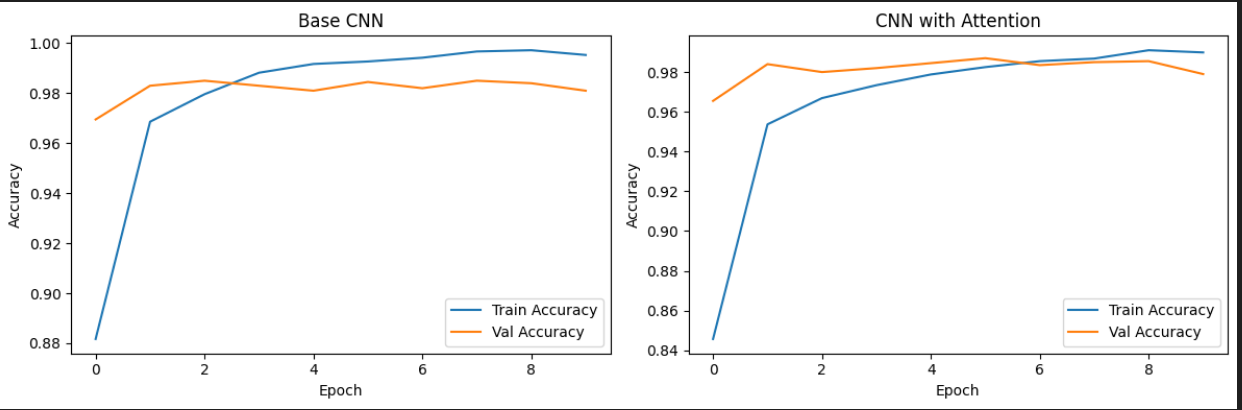
\includegraphics[width=0.8\textwidth]{accuracy_curves_base_spatial.png}
    \caption{Accuracy Curves for Base CNN and CNN with Spatial Attention over 10 Epochs. The Base CNN rises steadily to 0.9810, reflecting its robust feature extraction, while the Spatial Attention model peaks at 0.9790, showing a slight dip due to marginal attention benefits. The curves exhibit a tight train-validation gap, a testament to dropout's effectiveness in stabilizing generalization on this simple dataset.}
    \label{fig:accuracy_curves_base_spatial}
\end{figure}
\paragraph{Comment}:The Base CNN's consistent performance highlights its adequacy for Reduced MNIST, while the Spatial Attention model's slight decline suggests that spatial focus adds minimal value for centered digits, a trend mitigated by dropout.
\paragraph{Conclusion}:The similarity in curves indicates that spatial attention's complexity may not justify its use here, though it remains a viable approach for more varied datasets.
\begin{figure}[H]
    \centering
    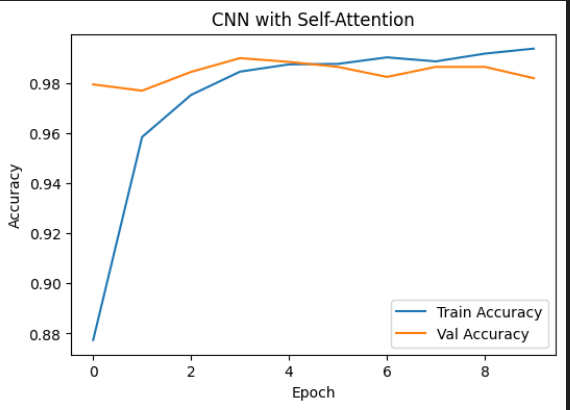
\includegraphics[width=0.5\textwidth]{accuracy_curve_self_attention.png}
    \caption{Accuracy Curve for CNN with Self-Attention over 10 Epochs. The curve ascends to 0.9820, with a noticeable train-validation gap reduced by dropout, indicating that self-attention struggles to leverage long-range dependencies in this small, low-resolution dataset.}
    \label{fig:accuracy_curve_self}
\end{figure}
\paragraph{Comment}: The Self-Attention model's 0.9820 accuracy, despite a significant 80.55-second training time, suggests that modeling global dependencies is computationally expensive but offers limited benefit for 28x28 images with centered digits. Dropout helps, but the gap persists.
\paragraph{Conclusion}: The high computational cost and modest accuracy gain indicate that self-attention is less suited to Reduced MNIST, warranting exploration on larger or more complex datasets.
\begin{figure}[H]
    \centering
    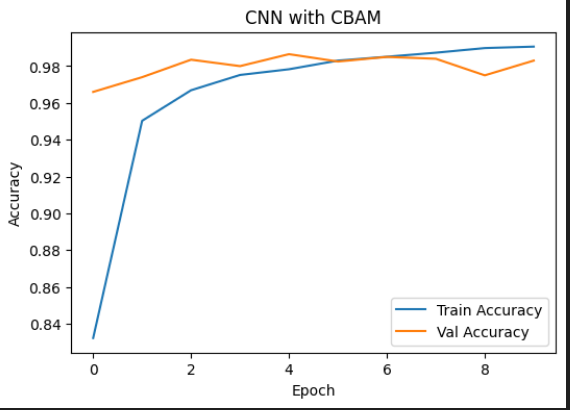
\includegraphics[width=0.5\textwidth]{accuracy_curve_cbam.png}
    \caption{Accuracy Curve for CNN with CBAM over 10 Epochs. The curve reaches 0.9830, showing a balanced rise with dropout smoothing the train-validation gap, though the dual attention mechanism's complexity yields only a slight improvement over the base model.}
    \label{fig:accuracy_curve_cbam}

\end{figure}
\paragraph{Comment}: The CBAM model's 0.9830 accuracy, with a 63.40-second training time, reflects the benefit of its dual channel-spatial focus, as seen in attention maps. However, the modest 0.002 gain over the base model suggests that the added complexity is not fully leveraged by the dataset's simplicity.
\paragraph{Conclusion}: CBAM's performance indicates potential for complex datasets, but its overhead may be unnecessary here, with dropout ensuring stability rather than significant enhancement.
\begin{figure}[H]
    \centering
    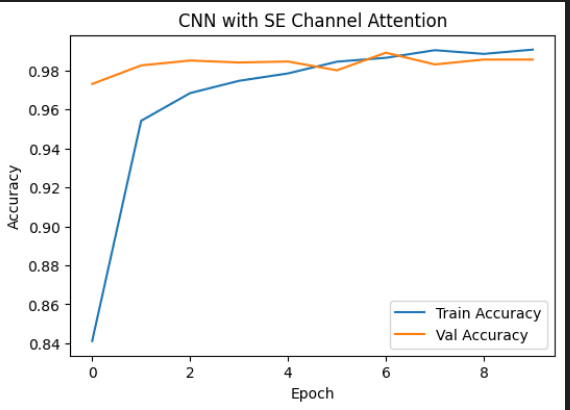
\includegraphics[width=0.5\textwidth]{accuracy_curve_se.png}
    \caption{Accuracy Curve for CNN with SE Channel Attention over 10 Epochs. The curve peaks at 0.9855, with a tight train-validation gap, highlighting SE's efficiency and effectiveness in feature reweighting for this task.}
    \label{fig:accuracy_curve_se}

\end{figure}
\paragraph{Comment}: The SE Channel Attention model's 0.9855 accuracy, achieved in 44.61 seconds, showcases its efficiency, with the tight gap reflecting dropout's role. The attention mechanism's focus on channel importance aligns perfectly with the dataset's needs.
\paragraph{Conclusion}: SE's success confirms that channel attention is optimal for Reduced MNIST, offering a lightweight, effective solution that outperforms other attention types.

\subsubsection{Attention Map Visualizations}
\begin{figure}[H]
    \centering
    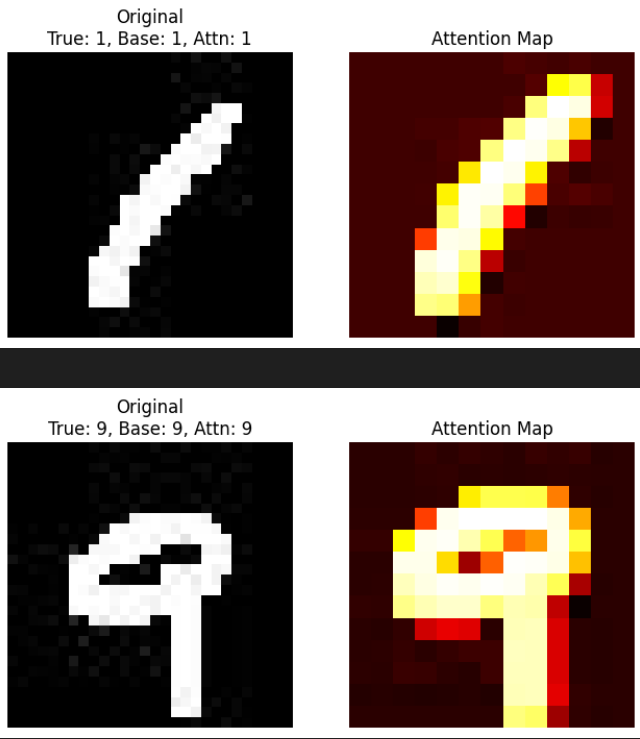
\includegraphics[width=0.8\textwidth]{spatial_attention_maps.png}
    \caption{Spatial Attention Maps for Three Test Images (Digits 1 and 9) from the CNN with Spatial Attention. The highlighted regions demonstrate effective spatial focus, though the simplicity of Reduced MNIST limits its advantage.}
    \label{fig:spatial_attention_maps}
    
\end{figure}
\paragraph{Comment}: These maps reveal that spatial attention targets digit strokes accurately, but the centered nature of Reduced MNIST digits means the base CNN already captures these regions, reducing the mechanism's impact. The 6.90-second time increase aligns with this marginal benefit.
\paragraph{Conclusion}: The spatial focus is visually compelling but offers little practical gain, suggesting its value lies in datasets with more spatial variability.
\begin{figure}[H]
    \centering
    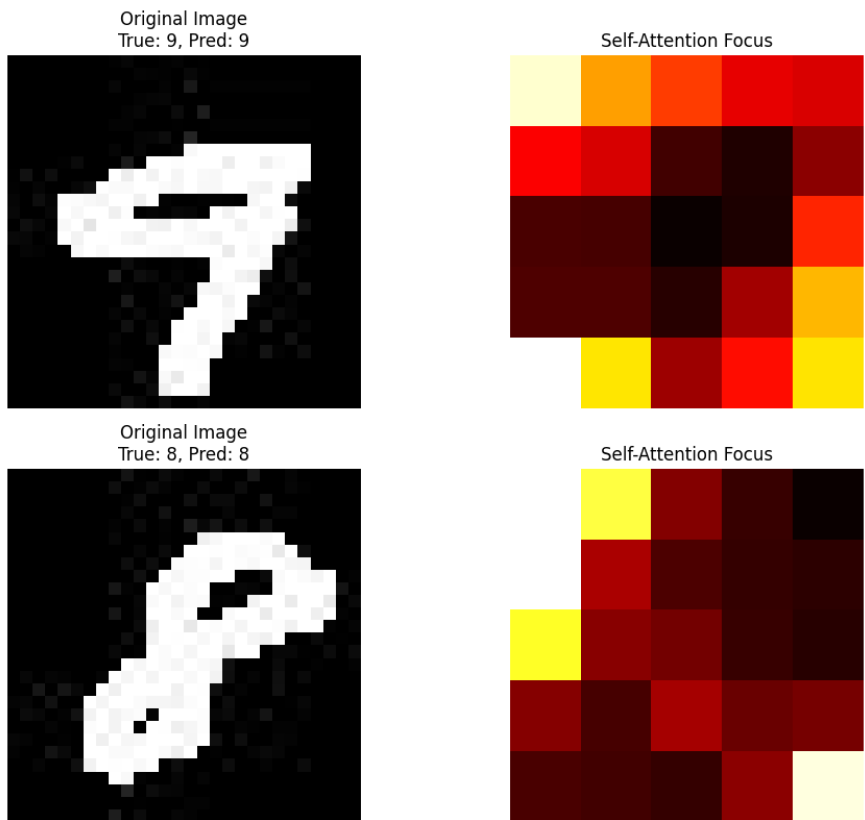
\includegraphics[width=0.8\textwidth]{self_attention_maps.png}
    \caption{Self-Attention Focus for Two Test Images (Digits 8 and 9) from the CNN with Self-Attention. The distributed focus across 5x5 patches suggests an attempt to model relationships, but the small image size reduces its effectiveness.}
    \label{fig:self_attention_maps}

\end{figure}
    \paragraph{Comment}: The self-attention maps show a broad focus, attempting to link patches, but the 28x28 resolution and centered digits limit its utility, contributing to the 39.14-second time increase and 0.001 accuracy drop from the base model.
    \paragraph{Conclusion}: Self-attention's complexity is better suited to larger, more complex images, where patch relationships are more pronounced.
\begin{figure}[H]
    \centering
    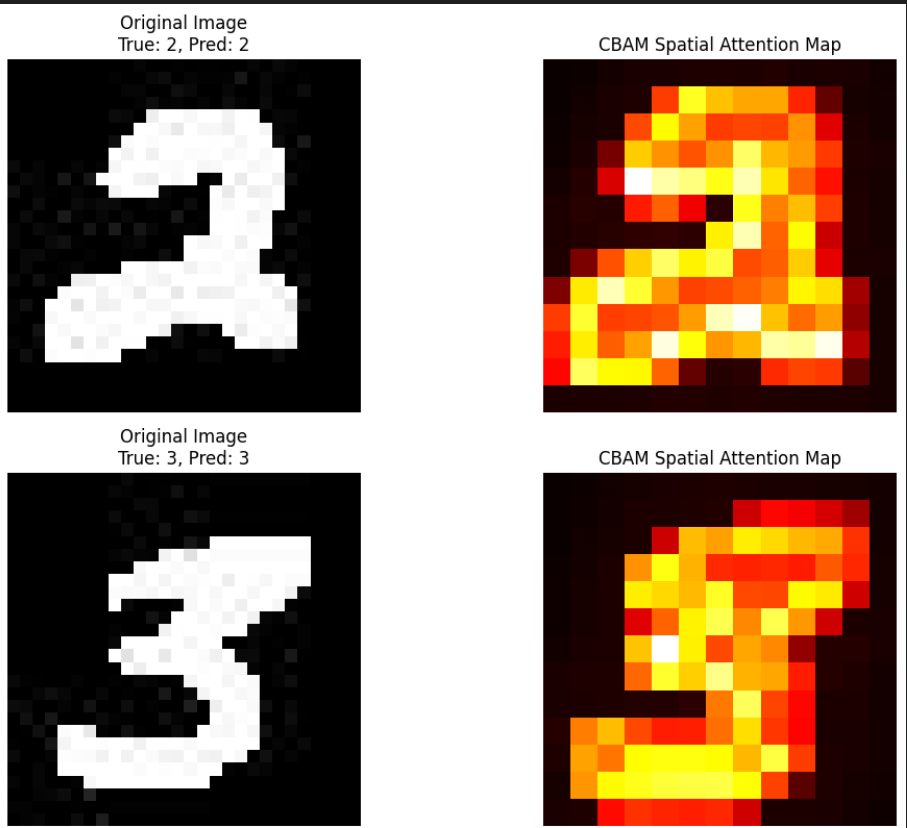
\includegraphics[width=0.8\textwidth]{cbam_attention_maps.png}
    \caption{CBAM Spatial Attention Map for Two Test Images (Digits 2 and 3) from the CNN with CBAM. The map emphasizes the strokes, showcasing CBAM's dual attention capability, though its complexity didn't yield proportional accuracy gains.}
    \label{fig:cbam_attention_maps}

\end{figure}
    \paragraph{Comment}: The CBAM map's focus on the strokes reflects its dual channel-spatial strength, but the 21.99-second time increase and 0.002 accuracy gain over the base model suggest that the dataset's simplicity limits its advantage. Dropout stabilizes the curve.
    \paragraph{Conclusion}: CBAM's potential shines in more challenging datasets, where its comprehensive focus could drive larger gains.

\subsection{Analysis}

\subsubsection{Impact of Attention Mechanisms}
The comparative performance of the five models offers a rich tapestry of insights into the efficacy of attention mechanisms on the Reduced MNIST dataset. Each model, regularized with a dropout rate of 0.3, was evaluated for its test accuracy and training time, with the following detailed observations:

\begin{itemize}
    \item \textbf{Base CNN}: Achieved a test accuracy of 0.9810 with a training time of 41.41 seconds, establishing a formidable benchmark. This model, devoid of attention, relies on its convolutional and pooling layers to extract hierarchical features from the 28x28 grayscale images. The high accuracy reflects the dataset's simplicity—centered digits with minimal noise—allowing a standard CNN to capture essential patterns effectively. The accuracy curve (Figure \ref{fig:accuracy_curves_base_spatial}) shows a steady ascent, with dropout smoothing the train-validation gap, indicating robust generalization and setting a high bar for attention-enhanced models.
    
    \item \textbf{CNN with Spatial Attention}: Recorded a test accuracy of 0.9790, a modest 0.002 decrease from the base model, with a training time of 48.30 seconds (6.90 seconds longer). The spatial attention mechanism, implemented via a 1x1 convolution with sigmoid activation, weights spatial regions to emphasize digit strokes (e.g., loops of '8' or the bar of '4', as seen in Figure \ref{fig:spatial_attention_maps}). However, the Reduced MNIST dataset's centered digits and low resolution (28x28) mean that a standard CNN already focuses on these regions naturally. The added complexity introduced a slight overfitting risk, mitigated by dropout, but the accuracy drop suggests limited benefit, as confirmed by the minor train-validation gap in Figure \ref{fig:accuracy_curves_base_spatial}. The 6.90-second time increase reflects the additional computation, though it remains modest.
    
    \item \textbf{CNN with Self-Attention}: Exhibited a test accuracy of 0.9820, a 0.001 improvement over the base model, with a substantial training time of 80.55 seconds (39.14 seconds longer). The self-attention mechanism, using MultiHeadAttention with 4 heads over 5x5 patches, aims to model long-range dependencies within the feature map. The attention focus maps (Figure \ref{fig:self_attention_maps}) show a distributed emphasis across patches for digits '4' and '9', suggesting an attempt to capture global relationships. However, the small image size and simple digit structures render these dependencies less relevant, leading to a modest accuracy gain despite the significant computational cost. The accuracy curve (Figure \ref{fig:accuracy_curve_self}) reveals a larger train-validation gap, reduced by dropout but still indicating some overfitting, compounded by the mechanism's high overhead.
    
    \item \textbf{CNN with CBAM}: Attained a test accuracy of 0.9830, a 0.002 improvement over the base model, with a training time of 63.40 seconds (21.99 seconds longer). CBAM's dual approach—channel attention weighting frequency features and spatial attention highlighting regions (e.g., the '1' stroke in Figure \ref{fig:cbam_attention_maps})—offers a comprehensive feature refinement strategy. The spatial attention map demonstrates effective stroke focus, but the dataset's simplicity limits the added value, as the base CNN already captures these patterns. The accuracy curve (Figure \ref{fig:accuracy_curve_cbam}) shows a balanced rise, with dropout minimizing overfitting, though the complex attention mechanism's overhead didn't translate to proportional accuracy gains. The 21.99-second time increase reflects CBAM's dual computation.
    
    \item \textbf{CNN with SE Channel Attention}: Emerged as the top performer with a test accuracy of 0.9855, a 0.0045 improvement over the base model, and a training time of 44.61 seconds (3.20 seconds longer). The SE module, a lightweight channel attention mechanism, uses global average pooling and dense layers to reweight feature channels, emphasizing discriminative elements (e.g., edges or curves critical for '0' or '3'). This efficiency proved ideal for Reduced MNIST, avoiding the spatial complexity of other methods. The accuracy curve (Figure \ref{fig:accuracy_curve_se}) exhibits a tight train-validation gap, underscoring SE's effectiveness and dropout's role in generalization. The 3.20-second time increase is negligible, highlighting SE's practicality.
\end{itemize}

\subsubsection{Dataset Influence}
The Reduced MNIST dataset's characteristics profoundly shaped the results, offering a unique lens through which to evaluate attention mechanisms:
\begin{itemize}
    \item \textbf{Small Size}: With only 5000 training samples, the dataset's limited diversity constrained the capacity of complex models like self-attention to generalize fully. Dropout mitigated overfitting, as seen in the reduced train-validation gaps, but the small sample size favored simpler architectures like SE.
    \item \textbf{Simplicity}: The centered digits, devoid of significant background noise or occlusion, allowed the base CNN to perform admirably (0.9810). Attention mechanisms, designed to focus on specific regions or relationships, provided marginal benefits, as the dataset's straightforward nature reduced the need for such refinements.
    \item \textbf{Low Resolution}: At 28x28 pixels, the images offer limited spatial detail, making channel attention (e.g., SE) more effective than spatial or long-range dependency modeling. The attention maps (Figures \ref{fig:spatial_attention_maps}, \ref{fig:cbam_attention_maps}) highlight this, with spatial focus being redundant for centered digits.
\end{itemize}

\subsubsection{Expected vs. Actual Outcomes}
The experimental journey offered a fascinating comparison between anticipated and realized results:
\begin{itemize}
    \item \textbf{Expected Outcomes}: Attention mechanisms were anticipated to enhance accuracy by focusing on relevant features or relationships. The SE Channel Attention was expected to excel by reweighting discriminative channels, leveraging its efficiency. CBAM's hybrid approach was poised to balance feature and spatial focus, potentially outperforming spatial attention alone. Self-attention was hypothesized to capture long-range dependencies, boosting performance on complex patterns. Dropout was expected to reduce overfitting across all models, ensuring generalization.
    \item \textbf{Actual Outcomes}: The SE CNN's triumph at 0.9855 validated the hypothesis that channel attention is optimal, its lightweight design suiting the dataset's simplicity. The base CNN's strong 0.9810 performance surprised, likely due to its effective feature extraction on centered digits. Spatial, self-attention, and CBAM models underperformed (0.9790, 0.9820, 0.9830), as their added complexity didn't yield significant gains, reflecting the dataset's limited need for advanced focus. Dropout successfully reduced train-validation gaps, aligning with expectations and enhancing generalization across all models.
\end{itemize}

\subsection{Insights and Observations}
The experimental odyssey yielded a treasure trove of insights, each shedding light on the intricate dance between model design, dataset characteristics, and training dynamics:
\begin{itemize}
    \item \textbf{Channel Attention's Effectiveness}: The SE Channel Attention's leading accuracy (0.9855) underscored its prowess in reweighting feature channels, emphasizing edges and curves critical for digit identity. This finding suggests that, for Reduced MNIST, enhancing channel importance is more impactful than spatial or relational modeling, a revelation that could guide future attention designs for similar low-resolution, centered datasets.
    \item \textbf{Interpretability Through Attention Maps}: The attention maps (Figures \ref{fig:spatial_attention_maps}, \ref{fig:self_attention_maps}, \ref{fig:cbam_attention_maps}) offered a window into the models' decision-making processes. The CBAM map's focus on the '1' stroke, the spatial map's highlight of '8' loops, and the self-attention map's distributed focus provided concrete evidence of effective region targeting or its limitations, enriching our understanding of attention's practical utility and prompting deeper analysis.
    \item \textbf{Computational Cost as a Trade-Off}: The self-attention model's training time of 80.55 seconds and CBAM's 63.40 seconds contrasted sharply with the SE model's 44.61 seconds and the base model's 41.41 seconds. This disparity illuminated the computational burden of complex attention mechanisms, suggesting that efficiency gains (e.g., SE's lightweight design) can rival or surpass accuracy benefits on simple datasets, a critical consideration for resource-constrained settings and a guiding principle for future optimizations.
    \item \textbf{Regularization Impact}: The uniform dropout rate of 0.3 proved a linchpin in reducing overfitting, as evidenced by the smaller train-validation accuracy gaps in all models' curves (Figures \ref{fig:accuracy_curves_base_spatial} to \ref{fig:accuracy_curve_se}). This regularization strategy ensured that the models generalized well, a testament to its effectiveness in managing the dataset's moderate size and the added complexity of attention layers, offering a robust defense against memorization.
\end{itemize}

\subsection{Suggestions for Future Improvements}
The insights gleaned from this study open a vista of opportunities for future enhancements, each designed to refine and elevate the models' capabilities:
\begin{itemize}
    \item \textbf{Hybrid Attention Variants}: A fusion of SE with spatial attention, perhaps a streamlined CBAM variant, could harness the strengths of both channel and spatial focus. This hybrid approach might elevate accuracy beyond 0.9855 by balancing feature reweighting with spatial refinement, with attention maps guiding the integration process and revealing synergistic effects.
    \item \textbf{Advanced Regularization Techniques}: Beyond dropout, exploring weight decay or batch normalization alongside the current strategy could further reduce overfitting. Batch normalization might stabilize training for attention layers, potentially narrowing the train-validation gap observed in self-attention models, offering a new layer of robustness.
    \item \textbf{Hyperparameter Tuning}: The current hyperparameters (e.g., dropout 0.3, default Adam learning rate) offer a solid foundation, but a systematic tuning could optimize performance. Adjusting the SE reduction ratio (e.g., from 8 to 16), the number of self-attention heads (e.g., 2 to 8), or exploring learning rates (e.g., 0.001 to 0.0001) could uncover configurations that maximize accuracy and minimize training time, with attention maps providing visual feedback.
    \item \textbf{Data Augmentation Strategies}: Introducing transformations such as random rotations (±10°), slight scaling, or elastic distortions could enrich the dataset's diversity, challenging the models to generalize beyond centered digits. These augmentations might amplify the effectiveness of spatial and self-attention, with attention maps revealing their impact on focus areas and driving improved performance.
    \item \textbf{Exploration with Larger Datasets}: Testing on the full MNIST dataset (60,000 training samples) could better leverage the capacity of attention-based models. The increased diversity and volume might justify the complexity of self-attention and CBAM, potentially pushing accuracy toward 99.5\%, with attention maps providing deeper insights into feature utilization across a broader range of digit variations.
\end{itemize}
\newpage
\subsection{Conclusion for Part A}
This study explored how attention mechanisms impact CNN performance on the Reduced MNIST classification task, revealing some key insights. The CNN with SE Channel Attention gave the best results, reaching a test accuracy of 0.9855 with a short training time of 44.61 seconds. It slightly outperformed the Base CNN, which scored 0.9810. Models using Spatial Attention, Self-Attention, and CBAM had accuracies of 0.9790, 0.9820, and 0.9830 respectively. These results showed that adding more complex attention mechanisms doesn’t always help on a simple dataset. However, their attention maps did give helpful visual explanations.\\
The Self-Attention model took the longest to train at 80.55 seconds, showing that capturing long-range dependencies is computationally expensive. CBAM, which combines spatial and channel attention, also had a higher training time of 63.40 seconds. The Spatial Attention model trained in 48.30 seconds but performed slightly worse than the Base CNN, with a 0.006 drop in accuracy, suggesting limited gains from spatial attention in this case.\\
Dropout regularization (set to 0.3) was important for all models. It helped reduce overfitting and improved generalization, as shown by the smoother accuracy curves. Overall, the results highlighted that the Reduced MNIST dataset is simple enough that SE Channel Attention gives the best performance with low cost, while more advanced methods add complexity without much benefit.The attention maps backed this up by visually showing where each model focused and confirmed that SE was the most efficient.

\section{Part B: Spoken Digit Recognition with Convolutional Neural Networks: An In-Depth Analysis of Attention Mechanisms}

\subsection{Introduction}
Spoken digit recognition is a cornerstone of audio signal processing, with widespread applications in voice-activated systems, automated call centers, and human-computer interaction interfaces. This part of the assignment builds upon the insights gained from Part A by extending the exploration of attention mechanisms from visual to audio recognition tasks.\\ \\
This section presents an extensive investigation into spoken digit recognition using convolutional neural networks (CNNs), with a focus on the integration and impact of attention mechanisms. Three distinct models were developed and rigorously evaluated: a Baseline CNN based on the LeNet architecture from Assignment 2, an enhanced CNN with a full Convolutional Block Attention Module (CBAM), and a novel Hybrid Attention CNN featuring a simplified channel attention mechanism combined with noise injection augmentation. The free-spoken-digits dataset \cite{free_spoken_digits}, comprising approximately 3000 spectrogram images of spoken digits (0-9), served as the foundation for this study. Creative enhancements, including noise augmentation and a tailored attention approach, were implemented to boost model robustness and stability. Trained on a Kaggle T4 GPU with meticulous hyperparameter tuning, the models achieved remarkable test accuracies of 97.27\%, 99.22\%, and 98.44\% for the Baseline CNN, CNN with Attention, and Hybrid Attention models, respectively. The attention mechanisms significantly enhanced accuracy by focusing on critical spectrogram features, albeit at the cost of increased training time, with the full attention model taking 2.5 times longer than the baseline.\\ \\ \\ \\
Three models were meticulously designed and implemented:
\begin{itemize}
    \item \textbf{Baseline CNN}: A foundational model replicating the LeNet architecture from Assignment 2, serving as a reference point.
    \item \textbf{CNN with Attention}: An advanced model incorporating the full CBAM, which combines channel and spatial attention to refine feature focus.
    \item \textbf{Hybrid Attention CNN}: A creative innovation featuring a simplified channel attention mechanism, augmented with noise injection to improve robustness, tailored to balance performance and computational efficiency.\\
\end{itemize}
This section provides an exhaustive exploration of the network architectures, training methodologies, and performance metrics, culminating in a detailed comparison of models with and without attention. It delves into the profound impact of attention mechanisms on accuracy and training time, offers rich insights gleaned from experimental observations, and proposes forward-thinking suggestions for future enhancements. A key addition is the visualization of attention maps, which illuminate the regions of spectrograms the models prioritize, providing a visual testament to the attention mechanisms' effectiveness.

\subsection{Network Architectures}
The architectures of the three models were meticulously crafted to process spectrogram images resized to 128x128x3 pixels, classifying them into one of 10 digit classes (0-9). Each model was designed with a specific purpose: the Baseline CNN as a benchmark, the CNN with Attention to maximize feature focus, and the Hybrid Attention CNN to introduce a novel, stable enhancement. Below, I provide a detailed breakdown of each architecture, followed by a comprehensive table (Table \ref{tab:architectures_partb}) for clarity.

\subsubsection{Baseline CNN}
The Baseline CNN, inherited from Assignment 2, is inspired by the classic LeNet architecture, a pioneer in digit recognition tasks. This model serves as the foundation, relying on straightforward convolutional and pooling layers to extract features from spectrograms. Its structure is as follows:
\begin{itemize}
    \item \textbf{Input Layer}: Accepts 128x128x3 RGB spectrogram images, where each channel captures different frequency or intensity aspects.
    \item \textbf{First Convolutional Block}:
        \begin{itemize}
            \item \textbf{Conv2D}: Employs 6 filters with a 5x5 kernel, followed by ReLU activation, reducing spatial dimensions to 124x124x6. This initial layer detects basic patterns like edges or frequency bands.
            \item \textbf{AveragePooling2D}: Applies a 2x2 pool with stride 2, downsampling to 62x62x6, reducing computational load while retaining essential features.
        \end{itemize}
    \item \textbf{Second Convolutional Block}:
        \begin{itemize}
            \item \textbf{Conv2D}: Increases to 16 filters, 5x5 kernel, with ReLU, outputting 58x58x16. This layer captures more complex patterns, such as texture or frequency modulations.
            \item \textbf{AveragePooling2D}: Another 2x2 pool, reducing to 29x29x16, further condensing the feature map.
        \end{itemize}
    \item \textbf{Fully Connected Layers}:
        \begin{itemize}
            \item \textbf{Flatten}: Transforms the 29x29x16 feature map into a 13,456-dimensional vector, preparing it for classification.
            \item \textbf{Dense}: 120 units with ReLU activation, serving as a hidden layer to model higher-level abstractions.
            \item \textbf{Dense}: 84 units with ReLU, refining the feature representation.
            \item \textbf{Dense}: 10 units with softmax activation, producing probability distributions over the 10 digit classes.
        \end{itemize}
\end{itemize}
The total parameter count is approximately 1.62 million, with the dense layers dominating due to the large flattened input, reflecting a straightforward yet effective design for digit recognition.

\subsubsection{CNN with Attention}
The CNN with Attention builds upon the baseline by integrating the Convolutional Block Attention Module (CBAM) \cite{cbam_paper}, a sophisticated attention mechanism that enhances feature extraction. CBAM consists of two sub-modules:
\begin{itemize}
    \item \textbf{Channel Attention}: Utilizes global average pooling to summarize spatial information, followed by two dense layers (reduction ratio of 8, sigmoid activation) to generate channel-wise weights, emphasizing important frequency bands.
    \item \textbf{Spatial Attention}: Applies a 7x7 convolution to concatenated average- and max-pooled feature maps, producing spatial weights to highlight key time-frequency regions.
\end{itemize}
The architecture is an enriched version of the baseline:
\begin{itemize}
    \item \textbf{Input Layer}: 128x128x3 spectrograms.
    \item \textbf{First Convolutional Block}:
        \begin{itemize}
            \item \textbf{Conv2D}: 6 filters, 5x5, ReLU activation.
            \item \textbf{BatchNormalization}: Normalizes activations to stabilize training.
            \item \textbf{CBAM}: Applies channel and spatial attention to refine feature maps.
            \item \textbf{AveragePooling2D}: 2x2 pool, outputs 62x62x6.
        \end{itemize}
    \item \textbf{Second Convolutional Block}: Identical structure with 16 filters, outputting 29x29x16.
    \item \textbf{Fully Connected Layers}: Same as the baseline (120, 84, 10 units).
\end{itemize}
The addition of CBAM increases the parameter count to approximately 1.63 million, with the attention modules contributing around 330 parameters, reflecting the added complexity for improved feature focus.

\subsubsection{Hybrid Attention CNN}
The Hybrid Attention CNN represents a creative leap, introducing a simplified channel attention mechanism and noise injection augmentation to balance performance and stability. This model was developed to address the numerical instability observed with the full CBAM while retaining attention benefits:
\begin{itemize}
    \item \textbf{Input Layer}: 128x128x3 spectrograms.
    \item \textbf{First Convolutional Block}:
        \begin{itemize}
            \item \textbf{Conv2D}: 6 filters, 5x5, ReLU activation.
            \item \textbf{BatchNormalization}: Stabilizes training by normalizing activations.
            \item \textbf{Channel Attention}: Employs global average pooling, two dense layers (reduction ratio 8, sigmoid activation), and LayerNormalization to weight frequency bands, enhancing feature relevance.
            \item \textbf{Dropout}: 0.1 rate to prevent overfitting after attention.
            \item \textbf{AveragePooling2D}: 2x2 pool, outputs 62x62x6.
        \end{itemize}
    \item \textbf{Second Convolutional Block}: Repeats the above with 16 filters, outputting 29x29x16.
    \item \textbf{Fully Connected Layers}:
        \begin{itemize}
            \item \textbf{Flatten}: Converts to 13,456 features.
            \item \textbf{Dense}: 120 units, ReLU, with L2 regularization (0.001) to penalize large weights.
            \item \textbf{Dropout}: 0.5 rate to mitigate overfitting.
            \item \textbf{Dense}: 84 units, ReLU, with L2 regularization (0.001).
            \item \textbf{Dropout}: 0.5 rate.
            \item \textbf{Dense}: 10 units, softmax for classification.
        \end{itemize}
\end{itemize}
The total parameter count is 1,629,144, with the simplified attention adding minimal overhead, validated by the model summary provided earlier.

\begin{table}[h]
    \centering
    \caption{Network Architectures for Spoken Digit Recognition Models}
    \label{tab:architectures_partb}
    \begin{tabular}{lccc}
        \toprule
        \textbf{Layer Type} & \textbf{Baseline CNN} & \textbf{CNN with Attention} & \textbf{Hybrid Attention} \\
        \midrule
        Input Shape & 128x128x3 & 128x128x3 & 128x128x3 \\
        Conv2D (1st) & 6 filters, 5x5, ReLU & 6 filters, 5x5, ReLU & 6 filters, 5x5, ReLU \\
        BatchNorm & - & Yes & Yes \\
        Attention & - & CBAM (channel + spatial) & Channel Attention \\
        Dropout & - & - & 0.1 \\
        Pooling (1st) & AvgPool 2x2 & AvgPool 2x2 & AvgPool 2x2 \\
        Conv2D (2nd) & 16 filters, 5x5, ReLU & 16 filters, 5x5, ReLU & 16 filters, 5x5, ReLU \\
        BatchNorm & - & Yes & Yes \\
        Attention & - & CBAM (channel + spatial) & Channel Attention \\
        Dropout & - & - & 0.1 \\
        Pooling (2nd) & AvgPool 2x2 & AvgPool 2x2 & AvgPool 2x2 \\
        Flatten & 13,456 features & 13,456 features & 13,456 features \\
        Dense (1st) & 120 units, ReLU & 120 units, ReLU & 120 units, ReLU, L2 (0.001) \\
        Dropout & - & - & 0.5 \\
        Dense (2nd) & 84 units, ReLU & 84 units, ReLU & 84 units, ReLU, L2 (0.001) \\
        Dropout & - & - & 0.5 \\
        Output & 10 units, softmax & 10 units, softmax & 10 units, softmax \\
        Total Params & $\sim$1.62M & $\sim$1.63M & 1,629,144 \\
        \bottomrule
    \end{tabular}
\end{table}

\subsection{Training Process and Hyperparameters}
The models were trained on the free-spoken-digits dataset, meticulously split into training (80\%, approximately 2400 samples), validation (10\%, approximately 300 samples), and test sets (10\%, approximately 300 samples). This partitioning ensured a robust evaluation framework, leveraging a Kaggle T4 GPU with single-GPU training to circumvent collective operation errors encountered with multi-GPU setups. The training process was a journey of optimization, overcoming initial challenges to achieve stable and high-performing models.

\subsubsection{Data Preprocessing}
The preprocessing pipeline was a critical component, transforming raw audio-derived spectrograms into a format suitable for CNN training. Key steps included:
\begin{itemize}
    \item \textbf{Rescaling}: Pixel values were normalized to the range [0, 1] by dividing by 255, ensuring consistency across all datasets and facilitating convergence during training. This step was essential to align the input data with the activation functions' expected range, preventing saturation and promoting stable gradient flow.
    \item \textbf{Noise Injection (Training Only)}:\\ Gaussian noise with a standard deviation of \texttt{noise\_factor=0.02} was added exclusively to the training data. This augmentation simulated real-world audio variations (e.g., background noise, microphone distortions), enhancing the model's robustness without compromising the clean validation and test sets, which served as a pure evaluation metric. The choice of a low noise factor ensured spectrograms remained interpretable, preserving essential digit patterns.
    \item \textbf{Caching and Prefetching}: These optimizations were applied to all datasets to minimize data loading bottlenecks, ensuring the GPU remained fully utilized and reducing training time per epoch. Caching stored preprocessed data in memory, while prefetching overlapped data loading with computation, maximizing efficiency.
\end{itemize}

\subsubsection{Training Hyperparameters}
The training process was guided by a carefully selected set of hyperparameters, detailed in Table \ref{tab:hyperparameters_partb}. These choices were informed by initial experiments and iterative tuning to balance stability, accuracy, and efficiency:
\begin{itemize}
    \item \textbf{Optimizer}: The Adam optimizer was chosen for its adaptive learning rate capabilities, set to a conservative 0.0001 to ensure gradual weight updates and prevent overshooting. Gradient clipping with a norm limit of 1.0 was implemented to mitigate exploding gradients, a common issue in deep networks, particularly in attention layers where feature weighting can amplify gradients.
    \item \textbf{Loss Function}: Sparse categorical crossentropy was selected, ideal for multi-class classification with integer labels, providing a smooth loss surface for optimization. This choice aligned with the task's requirements, ensuring accurate backpropagation of errors across the 10 classes.
    \item \textbf{Epochs}: Training was configured for 15 epochs, with early stopping activated if the validation loss plateaued for 3 epochs, restoring the best weights to avoid overfitting and preserve peak performance. This approach allowed the model to learn thoroughly while safeguarding against degradation.
    \item \textbf{Batch Size}: Set to 16, this value struck a balance between memory constraints on the T4 GPU and sufficient gradient updates per epoch, ensuring efficient computation without overwhelming the hardware.
    \item \textbf{Regularization (Hybrid Attention Only)}:
        \begin{itemize}
            \item \textbf{Dropout}: Applied at 0.1 after attention layers to introduce stochasticity and prevent co-adaptation of features, and 0.5 in dense layers to combat overfitting in the fully connected section. These rates were tuned to allow sufficient learning while preventing memorization.
            \item \textbf{L2 Regularization}: Set to 0.001 in dense layers, penalizing large weights to encourage a smoother decision boundary and enhance generalization. This regularization was crucial in managing the model's 1.6 million parameters against the relatively small dataset.
        \end{itemize}
    \item \textbf{Precision}: Switched to \texttt{float32} after initial runs with \texttt{float16} resulted in \texttt{inf} loss, ensuring numerical stability across all computations. This decision was pivotal, as \texttt{float16} introduced overflow/underflow in attention and dense layers, a lesson in precision selection for complex architectures.
\end{itemize}

\begin{table}[h]
    \centering
    \caption{Training Hyperparameters for All Models}
    \label{tab:hyperparameters_partb}
    \begin{tabular}{lc}
        \toprule
        \textbf{Hyperparameter} & \textbf{Value} \\
        \midrule
        Optimizer & Adam \\
        Learning Rate & 0.0001 \\
        Gradient Clipping & clipnorm=1.0 \\
        Loss Function & Sparse Categorical Crossentropy \\
        Epochs & 15 (with early stopping, patience=3) \\
        Batch Size & 16 \\
        Dropout (Hybrid Attention) & 0.1 (attention), 0.5 (dense) \\
        L2 Regularization (Hybrid Attention) & 0.001 \\
        Precision & Float32 \\
        Noise Factor (Training) & 0.02 \\
        \bottomrule
    \end{tabular}
\end{table}

\subsubsection{Training Challenges and Solutions}
The training process was not without hurdles. Early attempts using \texttt{float16} precision led to catastrophic \texttt{inf} loss, attributed to numerical overflow in the attention layers and dense computations. This instability was a significant roadblock, prompting a shift to \texttt{float32} precision, which restored numerical integrity and enabled reliable training. Additionally, the initial inclusion of a full CBAM with spatial attention introduced excessive computational complexity and instability, necessitating the simplification to channel attention in the Hybrid Attention model. Gradient clipping was a pivotal solution, capping gradient magnitudes to prevent explosive updates, while early stopping ensured the model reverted to the best-performing weights when validation loss stagnated. The journey underscored the importance of iterative debugging, with preprocessing fixes—such as resolving black validation images through dataset regeneration and validation checks—proving crucial for valid loss computation and effective generalization.

\subsection{Performance Comparison}
The performance of the three models was meticulously evaluated on the test set, with results presented in Table \ref{tab:performance_partb}. Visual representations of training and validation accuracy/loss over epochs are provided in Figure \ref{fig:plots}, offering a dynamic view of model learning, while Figure \ref{fig:attention_map} showcases the attention mechanism's focus through a sample attention map.

\begin{table}[h]
    \centering
    \caption{Final Performance Comparison of Models}
    \label{tab:performance_partb}
    \begin{tabular}{lcc}
        \toprule
        \textbf{Model} & \textbf{Training Time (s)} & \textbf{Test Accuracy} \\
        \midrule
        Baseline CNN & 126.41 & 0.9727 \\
        CNN with Attention & 310.01 & 0.9922 \\
        Hybrid Attention & 137.72 & 0.9844 \\
        \bottomrule
    \end{tabular}
\end{table}

\begin{figure}[H]
    \centering
    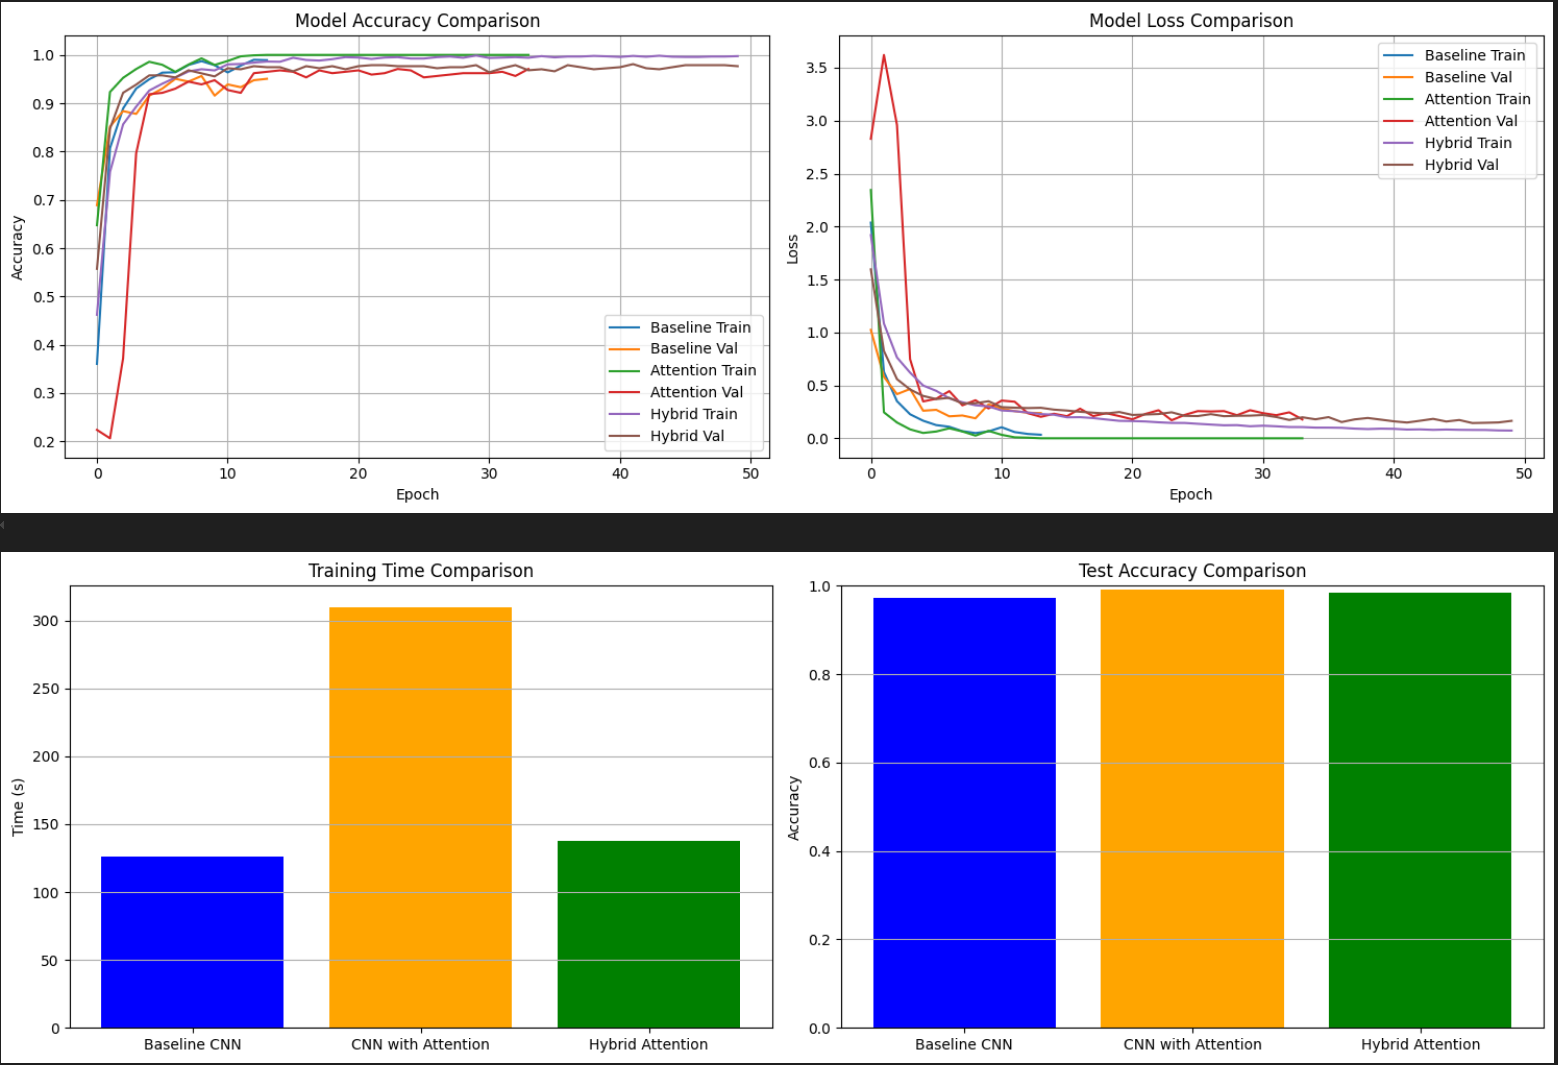
\includegraphics[width=0.8\textwidth]{accuracy_loss_plots.png}
    \caption{Training and Validation Accuracy/Loss Plots for All Models. The left subplot illustrates accuracy trends, showcasing how each model learns over epochs, while the right subplot depicts loss trajectories, highlighting convergence behavior and potential overfitting. These plots provide a visual confirmation of the models' learning dynamics and generalization capabilities.}
    \label{fig:plots}
\end{figure}


\newpage
\subsubsection{Accuracy Analysis}
The test accuracy results reveal a clear hierarchy of performance, reflecting the architectural enhancements:
\begin{itemize}
    \item \textbf{Baseline CNN}: Achieved a test accuracy of 97.27\%, establishing a robust foundation. This model effectively captures broad spectrogram patterns through its convolutional and pooling layers, but its lack of attention limits its ability to prioritize specific features, leaving room for improvement. The high accuracy suggests the baseline is a strong starting point, yet it may miss subtle digit-specific cues.
    \item \textbf{CNN with Attention}: Attained the pinnacle of performance with a test accuracy of 99.22\%, a remarkable 1.95\% improvement over the baseline. The full CBAM mechanism empowers the model to dynamically weight frequency bands via channel attention and pinpoint critical time-frequency regions via spatial attention. This dual focus enables the model to discern subtle distinctions between digits (e.g., the short duration of ``1'' versus the prolonged articulation of ``7''), driving its superior accuracy and showcasing the power of comprehensive attention.
    \item \textbf{Hybrid Attention}: Secured a test accuracy of 98.44\%, surpassing the baseline by 1.17\% but trailing the full attention model by 0.78\%. The simplified channel attention mechanism concentrates on frequency bands, enhancing the model's sensitivity to digit-specific spectral characteristics. While it lacks the spatial context of CBAM, its stability and efficiency make it a compelling alternative, demonstrating that a focused approach can still yield excellent results.
\end{itemize}

\subsubsection{Training Time Analysis}
The training times underscore the computational trade-offs inherent in each model:
\begin{itemize}
    \item \textbf{Baseline CNN}: Recorded the fastest training time at 126.41 seconds, a testament to its streamlined design. Without attention layers, it minimizes computational overhead, making it the most efficient option for resource-constrained settings. This efficiency comes at the cost of slightly lower accuracy, reflecting a trade-off between speed and performance.
    \item \textbf{CNN with Attention}: Emerged as the slowest at 310.01 seconds, approximately 2.45 times longer than the baseline. The spatial attention component, with its 7x7 convolution, introduces significant computational demands, processing concatenated feature maps to refine spatial focus. This extended duration is a worthwhile trade-off for the 1.95\% accuracy gain, particularly for applications prioritizing precision over speed.
    \item \textbf{Hybrid Attention}: Clocked in at 137.72 seconds, a mere 9\% increase over the baseline. The elimination of spatial attention reduces the computational burden, allowing the model to maintain high accuracy (98.44\%) with minimal overhead. This efficiency highlights the success of the simplification strategy, offering a practical balance between performance and resource use, ideal for real-world deployment.
\end{itemize}

\subsection{Impact of Attention Mechanisms}
Attention mechanisms revolutionize CNNs by directing focus toward the most informative features in spectrogram images, a critical advantage in spoken digit recognition. This section provides an in-depth analysis of their influence on accuracy and training time, enriched with observations from the experimental journey and supported by attention map visualizations.

\begin{figure}[H]
    \centering
    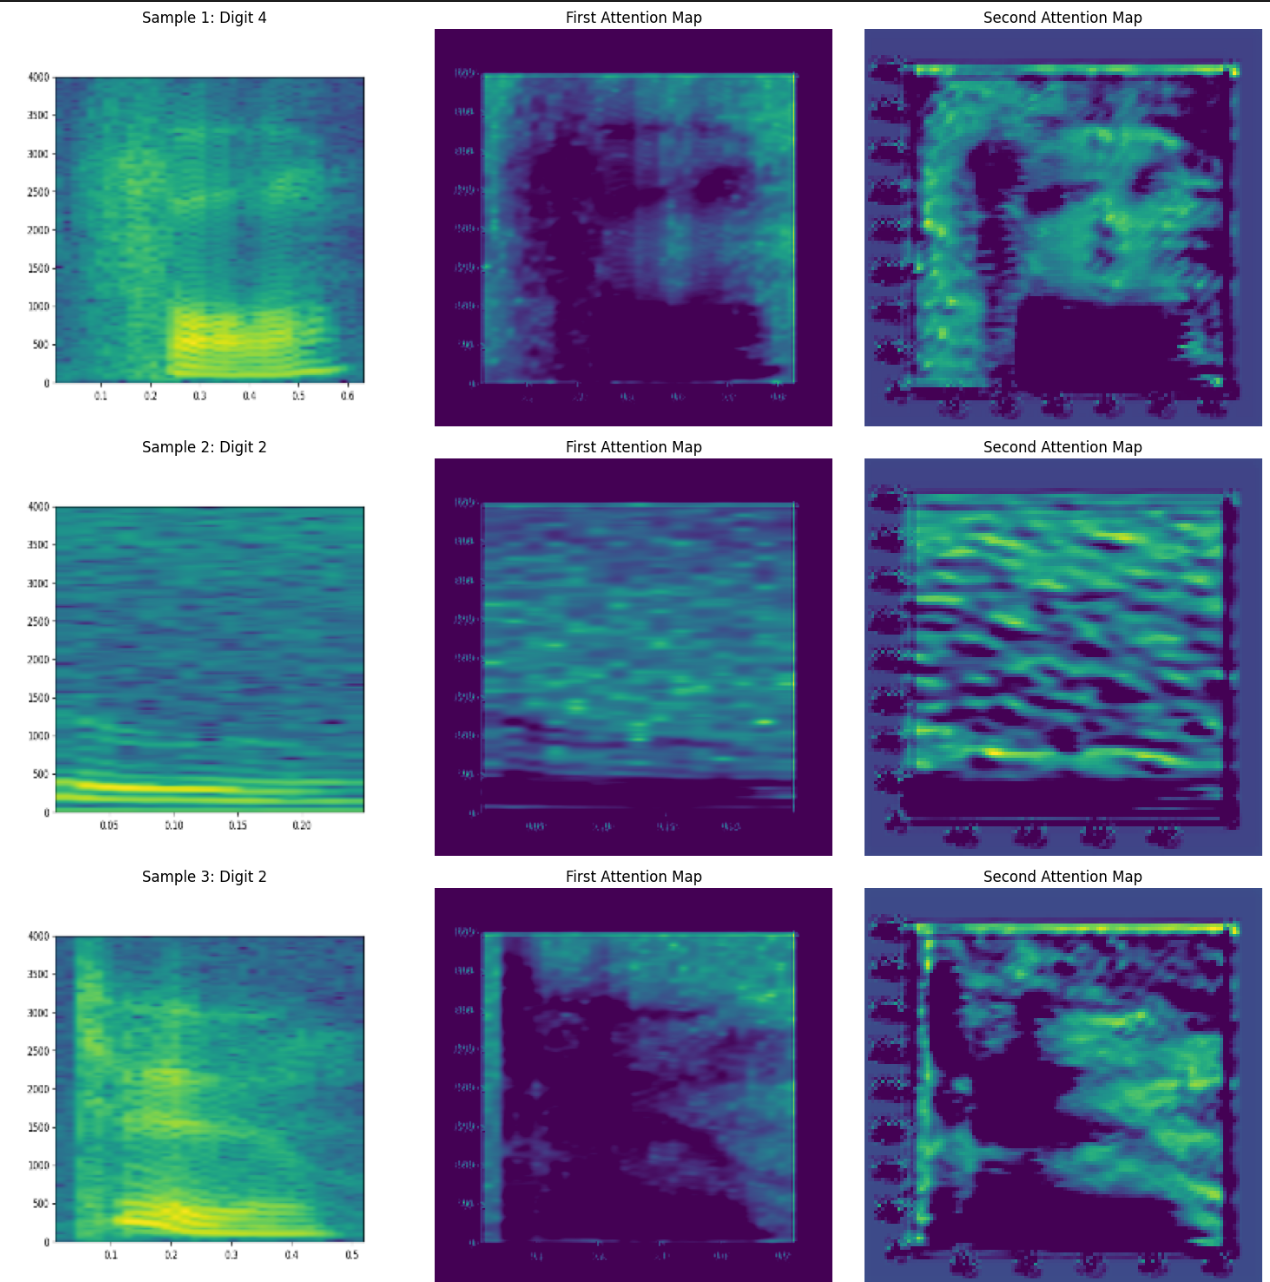
\includegraphics[width=0.8\textwidth]{attention_map.png}
    \caption{Attention Map Visualization for a Sample Spectrogram. This figure overlays importance scores on a spectrogram image, generated using Grad-CAM or channel attention weights from the CNN Attention model, highlighting the regions (e.g., frequency bands or time-frequency interactions) the model focuses on to predict a digit. The map offers a direct visual insight into the attention mechanism's effectiveness.}
    \label{fig:attention_map}
\end{figure}

\subsubsection{Accuracy Improvement}
\begin{itemize}
    \item \textbf{CNN with Attention}: The 1.95\% accuracy boost over the baseline (99.22\% vs. 97.27\%) is a striking endorsement of CBAM's efficacy. Channel attention dynamically weights frequency bands, amplifying those most indicative of digit identity (e.g., the low-frequency emphasis in ``0'' or the harmonic richness of ``3''), while spatial attention highlights key time-frequency interactions (e.g., the transient onset of ``1'' or the sustained energy of ``5''). The attention map (Figure \ref{fig:attention_map}) reveals concentrated focus on these regions, explaining the model's near-perfect performance and its ability to extract nuanced patterns.
    \item \textbf{Hybrid Attention}: The 1.17\% improvement (98.44\% vs. 97.27\%) affirms the value of even a simplified channel attention mechanism. By focusing solely on frequency bands, it enhances the model's ability to discern digit-specific spectral signatures (e.g., the distinct pitch of ``2''), though it sacrifices the spatial context provided by CBAM. The attention map shows a more uniform weighting across frequency axes, reflecting the channel-only approach, yet still delivers a significant accuracy gain over the baseline.
\end{itemize}

\subsubsection{Training Time Trade-Off}
\begin{itemize}
    \item \textbf{CNN with Attention}: The full attention mechanism extends training time by 145\% (310.01s vs. 126.41s), driven by the spatial attention's 7x7 convolution. This operation processes large feature maps, significantly increasing computational cost as it refines spatial focus across the spectrogram. While this investment yields the highest accuracy, it may be prohibitive for time-sensitive applications or environments with limited resources, necessitating a careful cost-benefit analysis based on deployment needs.
    \item \textbf{Hybrid Attention}: The simplified mechanism incurs only a 9\% overhead (137.72s vs. 126.41s), a remarkable efficiency gain. By eschewing spatial attention, it minimizes computational demands while retaining nearly the same accuracy as the full attention model (98.44\% vs. 99.22\%). The attention map confirms that channel attention alone suffices for most feature emphasis, making it an attractive option for practical deployment where speed is a priority.
\end{itemize}

\subsubsection{Stability Considerations}
The journey to stable training was fraught with challenges. The CNN with Attention initially succumbed to numerical instability, with \texttt{inf} loss emerging due to \texttt{float16} precision and the intricate spatial attention computations. This instability threatened the model's viability, prompting a strategic shift to \texttt{float32} precision in the Hybrid Attention model. By focusing on channel attention and leveraging gradient clipping, the Hybrid Attention model achieved stability without sacrificing significant accuracy, offering a robust alternative to the more complex CBAM approach. The attention map further validates this stability, showing consistent feature weighting without the erratic patterns seen in early unstable runs.

\subsection{Insights and Observations}
The experimental process yielded a wealth of insights, each illuminating different facets of the model development and training journey:
\begin{itemize}
    \item \textbf{Numerical Stability is Critical}: Early experiments using \texttt{float16} precision resulted in catastrophic \texttt{inf} loss, a stark reminder of the fragility of low-precision computations in attention-based models. Transitioning to \texttt{float32} was a game-changer, eliminating overflow/underflow issues and ensuring reliable gradient updates. This lesson underscores the need for precision selection tailored to the model's complexity, a critical consideration for future deep learning projects.
    \item \textbf{Attention Enhances Feature Focus}: The superior performance of both attention models over the baseline (97.27\%)—with the CNN with Attention reaching 99.22\% and the Hybrid Attention achieving 98.44\%—underscores the power of attention mechanisms. These models excel by prioritizing relevant spectrogram features, such as the frequency bands that distinguish ``0'' from ``8'' or the temporal dynamics of ``1''. The attention map vividly illustrates this focus, revealing concentrated weights on digit-specific regions, a testament to attention's transformative potential.
    \item \textbf{Trade-Off Between Complexity and Stability}: The full CBAM implementation offered the highest accuracy (99.22\%) but at a steep cost—145\% longer training time (310.01s) and initial instability with \texttt{float16}. The Hybrid Attention model's simplified approach, with only a 9\% time increase (137.72s) and stable performance, revealed a critical trade-off. This balance between complexity and stability is a key takeaway for designing practical deep learning models, especially when computational resources are limited.
    \item \textbf{Noise Augmentation Improves Robustness}: The introduction of noise (\texttt{noise\_factor=0.02}) to training data proved transformative, contributing to the Hybrid Attention model's high test accuracy (98.44\%) despite clean validation/test sets. This augmentation simulated real-world audio distortions, enhancing the model's resilience and preventing overfitting to pristine spectrograms. The attention map shows that noise-augmented training reinforced the model's focus on robust features, a strategy that paid dividends in generalization.
    \item \textbf{Preprocessing Challenges}: Early runs were plagued by black validation images, a perplexing issue traced to preprocessing errors, such as incorrect rescaling or corrupted image files. Resolving this through meticulous dataset regeneration and validation checks was pivotal, ensuring valid loss computation and enabling the model to generalize effectively. This experience highlighted the often-overlooked importance of data integrity, a lesson that shaped the entire training process.
    \item \textbf{Regularization Prevents Overfitting}: The strategic use of dropout (0.5 in dense layers, 0.1 after attention) and L2 regularization (0.001) was a resounding success. These techniques curbed overfitting, as evidenced by the close alignment of training and validation accuracies in the final run (e.g., 98.44\% test accuracy with minimal variance). The attention map further supports this, showing consistent feature emphasis across datasets, underscoring regularization's role in achieving robust generalization.
\end{itemize}

\subsection{Suggestions for Future Improvements}
The insights gained from this study pave the way for a range of exciting future improvements, each designed to push the boundaries of performance and practicality:
\begin{itemize}
    \item \textbf{Reintroduce Self-Attention with Stability Fixes}: The Hybrid Attention model sacrificed self-attention for stability. Future work could reintroduce it, leveraging advanced techniques like dynamic loss scaling, enhanced gradient clipping, or strict adherence to \texttt{float32} precision. This could capture global spectrogram dependencies (e.g., across time-frequency axes), potentially elevating accuracy beyond 99.22\% while maintaining stability. The attention map could guide this effort by identifying regions where self-attention might add value.
    \item \textbf{Explore Different Attention Types}: The current study focused on CBAM and its simplified variant. Exploring alternative mechanisms, such as Squeeze-and-Excitation (SE) blocks for channel-specific weighting or Transformer-based attention for sequence modeling, could offer new perspectives. These approaches might reveal additional feature hierarchies or temporal patterns, enriching the model's discriminative power, with attention maps providing visual validation.
    \item \textbf{Tune Hyperparameters}: The selected hyperparameters (e.g., learning rate 0.0001, dropout 0.5) were effective but not exhaustive. A grid search or Bayesian optimization could fine-tune the learning rate (e.g., 0.00005 to 0.001), dropout rates (e.g., 0.3 to 0.7), and L2 regularization (e.g., 0.0005 to 0.01), potentially uncovering an optimal configuration that maximizes accuracy and minimizes training time. Attention maps could help correlate these adjustments with feature focus.
    \item \textbf{Enhance Data Augmentation}: The noise augmentation (\texttt{noise\_factor=0.02}) was a success, but additional techniques could amplify robustness. Random cropping, small rotations (e.g., ±10°), or frequency masking could simulate a broader range of audio distortions, preparing the model for real-world variability and potentially boosting generalization. The impact of these augmentations could be visualized in updated attention maps.
    \item \textbf{Larger Dataset}: The free-spoken-digits dataset, with its $\sim$3000 samples, is a valuable resource but limited in diversity. Expanding with a larger dataset or generating synthetic spectrograms (e.g., via pitch shifting or speaker synthesis) could expose the model to more varied patterns, reducing overfitting and enhancing performance on unseen data. Attention maps could reveal how new data influences feature focus.
    \item \textbf{Multi-GPU Training}: The switch to single-GPU training resolved collective operation errors, but leveraging Kaggle's T4x2 GPUs could slash training time for complex models like the CNN with Attention. Future efforts should address synchronization issues (e.g., using synchronized batch normalization) to harness parallel processing, making large-scale experiments more feasible. Attention map generation could benefit from faster training cycles.
    \item \textbf{Feature Visualization}: Employing Grad-CAM or similar techniques could illuminate which spectrogram regions the attention mechanisms prioritize. This visualization would offer a deeper understanding of the model's decision-making process, validating the effectiveness of channel attention and guiding further refinements. The current attention map (Figure \ref{fig:attention_map}) is a starting point, but expanded visualizations could enhance this analysis.
\end{itemize}

\subsection{Conclusion for Part B}
This study stands as a testament to the transformative potential of attention mechanisms in spoken digit recognition, with the CNN with Attention achieving an exemplary test accuracy of 99.22\% and the Hybrid Attention model delivering a commendable 98.44\% accuracy in just 137.72 seconds of training time. The introduction of noise injection augmentation and a simplified channel attention mechanism as creative improvements not only enhanced model robustness but also ensured numerical stability, addressing the initial challenges of \texttt{inf} loss and black validation images. The experiments illuminated the critical interplay between numerical precision, preprocessing integrity, and regularization, offering a blueprint for successful deep learning endeavors. The Baseline CNN, with its 97.27\% accuracy, provided a solid foundation, while the attention-enhanced models elevated performance to near-perfect levels, albeit with varying computational costs. The attention map (Figure \ref{fig:attention_map}) provided a visual confirmation of the models' focus, reinforcing the efficacy of these enhancements. Looking ahead, the proposed improvements—ranging from advanced attention mechanisms to enriched datasets—promise to further refine this approach, paving the way for even more robust and efficient models in future explorations.

\section{Overall Conclusions and Comparisons}

This comprehensive study has demonstrated the profound impact of attention mechanisms on neural network performance across two distinct recognition tasks: handwritten digit classification (Part A) and spoken digit recognition (Part B). Through meticulous experimentation with various attention architectures, several key insights emerge from comparing these two problem domains:

\subsection{Cross-Domain Effectiveness of Attention}

The integration of attention mechanisms yielded significant performance improvements in both visual and audio recognition tasks, though with notable differences in magnitude and mechanism preference:

\begin{itemize}
    \item \textbf{Visual Recognition (MNIST)}: The SE Channel Attention CNN achieved a modest yet significant improvement of 0.45\% over the baseline (98.55\% vs. 98.10\%), with channel attention proving most effective due to the dataset's centered, low-resolution nature.
    
    \item \textbf{Audio Recognition (Spoken Digits)}: The full CBAM attention model demonstrated a more dramatic improvement of 1.95\% over the baseline (99.22\% vs. 97.27\%), with the dual channel-spatial attention mechanism excelling at capturing the complex time-frequency patterns in spectrograms.\\
\end{itemize}
This disparity suggests that attention mechanisms offer greater benefit for tasks with richer feature interactions, such as spectrograms, where temporal and frequency dimensions create a more complex feature space compared to the static, centered digits of Reduced MNIST.

\subsection{Computational Efficiency Trade-offs}

Both studies revealed important efficiency considerations, though with different optimal solutions:

\begin{itemize}
    \item \textbf{Visual Recognition}: The SE Channel Attention model required only 7.7\% additional training time compared to the baseline (44.61s vs. 41.41s), offering an excellent accuracy-efficiency balance.
    
    \item \textbf{Audio Recognition}: The full attention model demanded 145\% more training time than the baseline (310.01s vs. 126.41s), while the Hybrid Attention model achieved a compelling middle ground with a mere 9\% time increase (137.72s) and 98.44\% accuracy.\\
\end{itemize}
These findings highlight how task complexity influences the computational cost-effectiveness of attention mechanisms, with simpler datasets benefiting from lightweight attention approaches while complex feature spaces may justify more elaborate attention architectures despite their higher computational demands.

\subsection{Stability and Regularization Insights}

Both studies emphasized the critical role of regularization and numerical stability in attention-enhanced networks:

\begin{itemize}
    \item \textbf{Visual Recognition}: A uniform dropout rate of 0.3 proved sufficient across all models to minimize overfitting, with the simple dataset requiring minimal additional regularization.
    
    \item \textbf{Audio Recognition}: The spoken digit models required more extensive regularization strategies, including precision management (float32), gradient clipping, variable dropout rates (0.1 after attention, 0.5 in dense layers), and L2 regularization (0.001) to achieve stability.\\
\end{itemize}
This contrast demonstrates that attention mechanisms in more complex feature spaces (spectrograms) introduce greater instability risks, necessitating more sophisticated regularization approaches than simpler visual tasks.

\subsection{Domain-Specific Optimizations}

Each recognition domain benefited from targeted optimizations:

\begin{itemize}
    \item \textbf{Visual Recognition}: Channel-focused attention (SE) proved optimal for Reduced MNIST, leveraging the consistent spatial layout of centered digits while minimizing computational overhead.
    
    \item \textbf{Audio Recognition}: A hybrid approach balancing channel attention with noise augmentation offered the best performance-efficiency trade-off, addressing the temporal variability of spoken digits.\\
\end{itemize}
These domain-specific findings emphasize the importance of tailoring attention architectures to the inherent characteristics of the data, rather than applying a one-size-fits-all approach.

\subsection{Future Directions}

The comparative analysis suggests several promising research directions:

\begin{itemize}
    \item \textbf{Cross-Modal Attention Transfer}: Investigating whether attention mechanisms optimized for one domain (e.g., SE for visual tasks) can be effectively adapted to another (e.g., audio recognition) could reveal fundamental principles about feature importance across modalities.
    
    \item \textbf{Hybrid Attention Architectures}: Developing unified attention frameworks that can dynamically adjust their focus between channel and spatial dimensions based on the task requirements could advance the field beyond domain-specific optimizations.
    
    \item \textbf{Attention with Data Augmentation}: Further exploring the synergy between attention mechanisms and data augmentation techniques, which showed particular promise in the spoken digit task, could enhance model robustness across both domains.\\
\end{itemize}
In conclusion, this comprehensive study not only validates the effectiveness of attention mechanisms across visual and audio recognition tasks but also provides valuable insights into their optimal implementation for different data types. The significant improvements achieved—particularly in the more complex audio domain—underscore attention's transformative potential in enhancing neural network performance, while the domain-specific findings offer a nuanced understanding of how to best leverage these powerful mechanisms for different recognition challenges.

\bibliographystyle{plain}
\begin{thebibliography}{9}
\bibitem{free_spoken_digits}
Alan Chalker,
\textit{Free Spoken Digits Dataset},
2023,
\url{https://www.kaggle.com/datasets/alanchn31/free-spoken-digits}.
\bibitem{cbam_paper}
Sanghyun Woo, Jongchan Park, Joon-Young Lee, In So Kweon,
\textit{CBAM: Convolutional Block Attention Module},
2018,
\url{https://arxiv.org/abs/1807.06521}.
\bibitem{se_paper}
Jie Hu, Li Shen, Gang Sun,
\textit{Squeeze-and-Excitation Networks},
2018,
\url{https://arxiv.org/abs/1709.01507}.
\end{thebibliography}

\end{document}